\chapter{Θεωρητικό Υπόβαθρο}

Στο παρόν κεφάλαιο θα οικοδομήσουμε την απαραίτητη γνώση στην οποία βασίζεται η έρευνα των επόμενων ενοτήτων. Αρχικά, θα παρουσιαστούν συνοπτικά τα τεχνητά νευρωνικά δίκτυα \footnote{Από εδώ και στο εξής, με τον όρο \textquote{νευρωνικά δίκτυα} θα αναφερόμαστε στα \textquote{τεχνητά νευρωνικά δίκτυα}.} υπό μια μαθηματική σκοπιά. Έπειτα, θα αναλυθούν τα \hyperlink{_capsule_networks}{νευρωνικά δίκτυα με κάψουλες} (\hyperlink{_capsule_networks}{\en{capsule networks}}) τα οποία και αποτελούν το κύριο θέμα της εργασίας. Τέλος, θα γίνει αναφορά σε νέες τεχνικές και αλγορίθμους που χρησιμοποιήθηκαν στο παρόν έργο ώστε η μετέπειτα εισαγωγή των μεθόδων μας για την εξέλιξη των νευρωνικών δικτύων με κάψουλες να είναι περισσότερο ομαλή και κατανοητή.

\section{Τεχνητά Νευρωνικά Δίκτυα}
Τα σημερινά τεχνητά νευρωνικά δίκτυα, όπως είναι αναμενόμενο, απέχουν σημαντικά από το πρώτο μοντέλο των \en{Warren McCulloch} και \en{Walter Pitts} \cite{mcculloch1943logical} που συζητήσαμε στην ενότητα \ref{sec:historic_note}. Με την ωρίμανση της τεχνολογίας, αυτή ανεξαρτητοποιήθηκε από την \hyperlink{_computational_neuroscience}{(υπολογιστική) νευροεπιστήμη} και εντάχθηκε στην Τεχνητή Νοημοσύνη υπό μια ιεραρχική δομή. Κρίνεται λοιπόν σκόπιμο να παρουσιάσουμε αυτήν την ιεραρχική δομή οργάνωσης της Τεχνητής Νοημοσύνης και μετέπειτα να αναφερθούμε στα επιμέρους στοιχεία της.
\par

\begin{figure}[h]
    \centering
    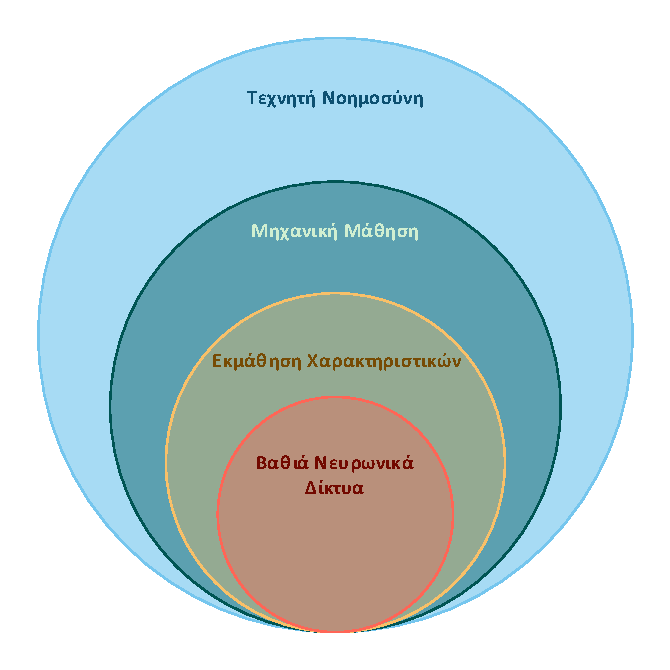
\includegraphics[width=0.7\textwidth]{images/chapter theoritical background/venn ai diagram thesis in greek new 2.pdf}
    \caption{Διάγραμμα \en{Venn} όπου απεικονίζει τη θέση των νευρωνικών δικτύων στην οργάνωση της τεχνητής νοημοσύνης. \textit{Παράχθηκε από το \href{https://www.microsoft.com/en-gb/microsoft-365/visio/flowchart-software/}{\en{Microsoft Visio\texttrademark}.}} }
    \label{fig:_venn_ai}
\end{figure}

Όπως βλέπουμε στο σχήμα \ref{fig:_venn_ai} τα νευρωνικά δίκτυα πολλών επιπέδων (βαθιά νευρωνικά δίκτυα) είναι ένα μέρος του κλάδου της εκμάθησης χαρακτηριστικών (\en{feature learning} ή \en{representation learning}) που είναι ένα μέρος της μηχανικής μάθησης η οποία με τη σειρά της ανήκει στο ευρύτερο επιστημονικό πεδίο της τεχνητής νοημοσύνης. Φυσικά, η τεχνητή νοημοσύνη περιλαμβάνει αρκετούς άλλους κλάδους εκτός από αυτόν της μηχανικής μάθησης\footnote{Βέβαια, ο κλάδος της μηχανικής μάθησης είναι σήμερα ο γρηγορότερα αναπτυσσόμενος.}. Μια χρήσιμη παρατήρηση είναι ότι οι σχέσεις υποσυνόλου συμπίπτουν με τη χρονική αλληλουχία ανάπτυξης του κάθε κλάδου. Δηλαδή, κάθε υποσύνολο αναπτύχθηκε ταυτόχρονα ή αργότερα από το οποιοδήποτε υπερσύνολό του.
\par
Στη συνέχεια, θα γίνει λόγος για τα στοιχεία εκείνα που περιλαμβάνουν την τεχνολογία των βαθιών νευρωνικών δικτύων προκειμένου ο αναγνώστης να αποκτήσει μια εποπτικότερη εικόνα.

\subsection{Μηχανική Μάθηση}


Όπως προδίδει ο όρος, σε αδρές γραμμές τα συστήματα μηχανικής μάθησης έχουν τη δυνατότητα να μαθαίνουν μια εργασία χωρίς να έχουν προγραμματιστεί με ρητές εντολές για τη συγκεκριμένη εργασία αυτή\footnote{Η δυνατότητα αυτή είναι πολύ σημαντική αφού, όπως διαπιστώσαμε στην ενότητα \ref{sec:historic_note} όταν έγινε λόγος για τα έμπειρα συστήματα, για πολλές εργασίες είναι πρακτικός αδύνατο να περιγραφούν ρητά και ντετερμινιστικά οι λύσεις τους.}. Ίσως, ο πιο πλήρης ορισμός δίνεται από τον \en{Tom M. Mitchell} \cite{mitchell1997machine} σύμφωνα με τον οποίο, ένα υπολογιστικό πρόγραμμα λέγεται ότι μαθαίνει από μια εμπειρία \en{E}, ως προς ένα σύνολο εργασιών \en{T} και ένα μέτρο απόδοσης \en{P}, εάν η απόδοσή του σε εργασίες του \en{T}, όπως αυτή μετριέται από το \en{P}, βελτιώνεται με την \en{E}. \footnote{Ο ορισμός αυτός εξηγεί γιατί για παράδειγμα η λήψη μιας ιστοσελίδας της βικιπέδιας και η αποθήκευσή της τοπικά στον υπολογιστή δεν αποτελεί μηχανική μάθηση. Όπως προκύπτει, η \textquote{γνώση} αυτή δεν καθιστά καλύτερο τον υπολογιστή σε κάποια εργασία\cite{geron2019hands}.}
\par

Σύμφωνα με τον ανωτέρω ορισμό διακρίνουμε τρία βασικά συστατικά ενός συστήματος μηχανικής μάθησης. Αυτά είναι τα παρακάτω:
\begin{description}
\item [Εργασία - \en{T}] Είναι το πρόβλημα το οποίο επιθυμούμε να λύσουμε.
\item [Μέτρο Απόδοσης - \en{P}] Αποτελεί μια μετρική του στόχου ως ένδειξη ποιότητας της λύσης μας. Από μαθηματική σκοπιά, είναι αυτό που ο αλγόριθμος μάθησης βελτιστοποιεί.
\item [Εμπειρία - \en{E}] Πρόκειται για τα δεδομένα εισόδου που λαμβάνει το σύστημα υπό τη μορφή παραδειγμάτων ή ως ερεθίσματα ανάδρασης από το περιβάλλον. Όπως θα δούμε στη συνέχεια, ο τρόπος απόκτησης αυτών των δεδομένων αλλά και η φύση τους καθορίζει το είδος της μάθησης.
\end{description}

\subsubsection{Βασικά Είδη Συστημάτων Μηχανικής Μάθησης}
\label{sec:_ML_varieties}
Τα είδη των συστημάτων μηχανικής μάθησης μπορούν να ταξινομηθούν ανάλογα με το:
\begin{itemize}
    \item \emph{Αν εκπαιδεύονται με ανθρώπινη επίβλεψη.}\\
    Ανάλογα με αυτό το κριτήριο έχουμε τις εξής βασικές κατηγορίες: επιβλεπόμενη (\en{supervised}), μη-επιβλεπόμενη (\en{un-supervised}) και ενισχυτική μάθηση (\en{reinforcement learning}).
    \item \emph{Αν μαθαίνουν σταδιακά (\en{incrementally}) και \textquote{στον αέρα} (\en{on the fly}).}\\
    Σε αυτήν την περίπτωση χωρίζουμε τα συστήματα μηχανικής μάθησης σε αυτά που πραγματοποιούν μάθηση σε ζωντανό χρόνο (\en{online learning}) και σε αυτά που μαθαίνουν κατά δέσμες (\en{batch learning}).
    \item \emph{Αν κατασκευάζουν μοντέλα προσαρμοσμένα στα δεδομένα.}\\ 
    Με αυτό το κριτήριο χωρίζονται σε συστήματα βασισμένα σε μοντέλο (\en{model-based}) ή σε συστήματα βασισμένα σε παραδείγματα (\en{instance-based}). \cite{geron2019hands}
\end{itemize}

Προφανώς, κάθε δυνατός συνδυασμός των παραπάνω κριτηρίων είναι αποδεκτός, οδηγώντας έτσι στην ταξινόμηση των συστημάτων μηχανικής μάθησης σε μια πληθώρα από διαφορετικές κατηγορίες. Κρίνεται χρήσιμο, να αναφέρουμε σε όλη την έκταση του έργου τις κατηγορίες στις οποίες ανήκει το κάθε σύστημα που παρουσιάζουμε. Για αυτόν τον λόγο, παροτρύνουμε τον αναγνώστη που δεν είναι εξοικειωμένος με τους ανωτέρω όρους να διαβάσει τους αντίστοιχους ορισμούς στο παράρτημα \ref{chap:definitions}. 
\subsection{Εκμάθηση Χαρακτηριστικών}
Η ανάπτυξη των πρώτων συστημάτων μηχανικής μάθησης απεμπόλησε την ανάγκη των ευφυών εφαρμογών για σχολαστική και ρητή (\en{hard-coded}) αναπαράσταση του χώρου του προβλήματος (π.χ. με την χρήση προτασιακής λογικής). Με τα νέα συστήματα, η γνώση για το πρόβλημα μαθαίνονταν αυτοματοποιημένα μέσω αλγορίθμων μάθησης από το σύνολο δεδομένων εκπαίδευσης. Με άλλα λόγια, τα αλγοριθμικά κατασκευάσματα μάθαιναν να αντιστοιχίζουν με αυτοματοποιημένο τρόπο τα δεδομένα εισόδου (κωδικοποιημένα σε μια μορφή αναπαράστασης) σε τιμές εξόδου. \par

Παρόλα αυτά, τα πρώτα, απλά συστήματα μηχανικής μάθηση δεν έλυσαν όλα τα προβλήματα. Όπως είναι εμφανές από την ανωτέρω περιγραφή, αν και δεν απαιτούνταν η λεπτομερή συγγραφή βάσεων γνώσης, παρέμενε η ανάγκη για αναπαράσταση των δεδομένων εισόδου με μια αποδοτική μορφή. Είναι γεγονός, άλλωστε, ότι η αναπαράσταση σε πολλά συστήματα επηρεάζει καθοριστικά την απόδοση του συστήματος\footnote{Η σημασία της αναπαράστασης δεδομένων στην απόδοση των αλγοριθμικών κατασκευασμάτων δε θα πρέπει να μας εκπλήσσει αφού κάτι αντίστοιχο ισχύει και στους ανθρώπους. Για παράδειγμα, οι περισσότεροι είναι πολύ πιο αποδοτικοί στην αριθμητική χρησιμοποιώντας την αραβική αναπαράσταση αριθμών απ ότι τη λατινική \cite{goodfellow2016deep}.}. Για αυτόν τον λόγο, εξελίχθηκαν διαδικασίες \textquote{μηχανικής χαρακτηριστικών} (\en{feature engineering}) όπου αξιοποιώντας την τεχνική γνώση του χώρου του προβλήματος (\en{domain knowledge}) στόχος είναι η αναπαράσταση των ακατέργαστων δεδομένων εκπαίδευσης ως σύνολο (συνήθως διάνυσμα) από κατάλληλα χαρακτηριστικά. Η καταλληλότητα έγκειται στο πόσο χρήσιμη πληροφορία παρέχουν τα χαρακτηριστικά υπό τον περιορισμό να είναι όσο το δυνατόν περισσότερο ανεξάρτητα μεταξύ τους ώστε να αποπλέκουν (\en{disentagle}) τους παράγοντες διακύμανσης (\en{factors of variation}) των δεδομένων που επηρεάζουν την τιμή εξόδου\cite{goodfellow2016deep}. \par

Οι ανωτέρω έννοιες μπορούν να καταστούν περισσότερο κατανοητές με ένα παράδειγμα συστήματος εκτίμησης τιμών κατοικιών\cite{geron2019hands} (πρόβλημα παλινδρόμησης, επίλυση με επιβλεπόμενη μάθηση κατά δέσμες). Πιο συγκεκριμένα, δοθέντος ενός συνόλου ακατέργαστων δεδομένων που αφορούν την αγορά σπιτιών σε μια περιοχή, το σύστημα, μέσω μηχανικής μάθησης, θα είναι ικανό να εκτιμήσει την τιμή με την οποία μια κατοικία θα πρέπει να κοστολογηθεί για να βγει στην αγορά. ;;Όπως εξηγήσαμε, προτού τροφοδοτήσουμε το σύστημα με το σύνολο δεδομένων, είναι σκόπιμο να εφαρμόσουμε διαδικασίες μηχανικής χαρακτηριστικών σε αυτά και να δημιουργήσουμε μια νέα αναπαράσταση. Τα ακατέργαστα δεδομένα εκπαίδευσης αποτελούνται από μια λίστα όπου κάθε γραμμή αντιστοιχεί σε μια οικία με όλες τις προδιαγραφές της και την τιμή πώλησής της. Στο πρόβλημα του παραδείγματος:
\begin{itemize}
    \item  Ένας παράγοντας διακύμανσης θα μπορούσε να είναι η ακρίβεια της συγκεκριμένης περιοχής. Εντούτοις, σαν προδιαγραφές ας υποθέσουμε ότι αναφέρονται μόνο το γεωγραφικό πλάτος και γεωγραφικό μήκος με αποτέλεσμα η ακρίβεια της περιοχής να μην είναι άμεσα παρατηρήσιμη (συνηθισμένο φαινόμενο στους παράγοντες διακύμανσης). Θα μπορούσαμε λοιπόν να μετατρέψουμε τις συντεταγμένες σε ένα νέο χαρακτηριστικό: την \textquote{κλάση} της περιοχής. Ένας ακόμα παράγοντας διακύμανσης που είναι όμως άμεσα παρατηρήσιμος είναι το εμβαδόν επιφάνειας της κατοικίας.
 \item Μη χρήσιμη πληροφορία θα μπορούσε να είναι ο προσανατολισμός της οικίας. Σε αυτή την περίπτωσή, η δημιουργία μιας νέας αναπαράσταση δεδομένων χωρίς το παρόν προσδιορισμό θα βοηθούσε την επίδοση του συστήματος. 
 \item Δύο αλληλοεξαρτώμενα χαρακτηριστικά (με υψηλή συν\textemdash διακύμανση) θα μπορούσαν να είναι ο αριθμός των υπνοδωματίων και ο αριθμός των μπάνιων όπου τότε η επιλογή της συγχώνευσής τους πιθανότατα βελτίωνε την απόδοση. 
\end{itemize}
\par

\begin{figure}[h]
  \centering
  
\includegraphics[width=0.95\textwidth]{images/chapter theoritical background/hog_gr.pdf}
  \caption{Παράδειγμα εξαγωγής χαρακτηριστικών σε εικόνα ενός αυτοκινήτου με τη μέθοδο του Ιστογράμματος Προσανατολισμένων Κλίσεων (\en{Histogram of Oriented Gradients}). \textit{Παράχθηκε τοπικά. TODO}} 
  \label{fig:_hog}
\end{figure}

Αν και στο παραπάνω πρόβλημα ήταν σχετικά εύκολη η \textquote{χειρονακτική} εξαγωγή χαρακτηριστικών, υπάρχουν πολλοί χώροι προβλημάτων όπου κάτι τέτοιο είναι από πολύ απαιτητικό έως απίθανο. Ενδεικτικά, σε ένα πρόβλημα οπτικής αναγνώρισης ζώων και αντικειμένων (όπως αυτό του \en{CIFAR-10}\cite{krizhevsky2009learning}) είναι εξαιρετικά δύσκολη η περιγραφή χαρακτηριστικών που θα λαμβάνουν μια αναπαράσταση σε εικονοστοιχεία (\en{pixel}) και θα παράγουν μια χρήσιμη αναπαράσταση. \par

Η λύση για την αντιμετώπιση των προβλημάτων της χειρονακτικής εξαγωγής χαρακτηριστικών είναι η χρήση των αλγορίθμων μηχανικής μάθησης για την εκμάθηση όχι μόνο για της αντιστοίχησης των δεδομένων εκπαίδευσης στην επιθυμητή έξοδο αλλά και των ίδιων των αναπαραστάσεων των δεδομένων. Αν και συνήθως, οι προκύπτουσες αναπαραστάσεις μετά τον μετασχηματισμό των ακατέργαστων δεδομένων δεν είναι κατανοητές από τον άνθρωπο, εφόσον η εκπαίδευση γίνει επιτυχημένα, αποτελούνται από χρήσιμα χαρακτηριστικά (που κωδικοποιούν τους παράγοντες διακύμανσης).
Χαρακτηριστικό παράδειγμα συστήματος για την εκμάθηση χαρακτηριστικών είναι ο Αυτοκωδικοποιητής (\en{Autoencoder}).

\subsection{Πολυεπίπεδα Νευρωνικά Δίκτυα}

Η εκμάθηση χαρακτηριστικών σε συνδυασμό με τις ιδέες του κονεκτιβισμού περί κατανεμημένης αναπαράστασης (βλ. ενότητα \ref{sec:historic_note}) μας οδηγεί αναπόφευκτα στη βαθιά μάθηση (\en{deep learning}). Υπό μια αφαιρετική σκοπιά, πρόκειται για τα λεγόμενα \textquote{πολυεπίπεδα νευρωνικά δίκτυα} τα οποία συνδυάζουν τόσο τον μετασχηματισμό της αναπαράστασης των δεδομένων εισόδου όσο και την αντιστοίχηση αυτών των νέων αναπαραστάσεων στην τιμή εξόδου. Τα συστήματα αυτά, όπως θα δούμε στη συνέχεια, είναι δομημένα από απλές υπολογιστικές μονάδες που τους επιτρέπουν να δημιουργούν σύνθετες αναπαραστάσεις μέσω μιας σειράς από εμφωλευμένες, απλούστερες αναπαραστάσεις. Σημειώνουμε ότι πραγματοποιούν μάθηση με κατασκευή μοντέλου (\en{model\textendash based learning systems}) και χρησιμοποιούνται τόσο σε προβλήματα ταξινόμησης όσο και παλινδρόμησης. Στις επόμενες παραγράφους, θα περιγράψουμε με μεγαλύτερη λεπτομέρεια τον χώρο των νευρωνικών δικτύων\footnote{Για έναν τυπικό ορισμό, παραπέμπουμε τον αναγνώστη στο παράρτημα \ref{chap:definitions}}.

\subsubsection{Δομή Απλών Νευρωνικών Δικτύων}
\label{sec:_vanilla_nn}
Τα Νευρωνικά Δίκτυα στην πιο βασική τους μορφή (\en{Feedforward Neural Networks} ή \en{Multilayer Perceptron}) αποτελούνται από απλούς τεχνητούς νευρώνες διασυνδεδεμένους μεταξύ τους με συνάψεις σχηματίζοντας μια πολυεπίπεδη διάταξη. Το πρώτο επίπεδο ονομάζεται επίπεδο εισόδου (\en{input layer}) ενώ το τελευταίο ονομάζεται επίπεδο εξόδου (\en{output layer}). Όλα τα ενδιάμεσα επίπεδα λέγονται κρυφά επίπεδα (\en{hidden layers}) διότι οι τιμές τους δε δίνονται από τα δεδομένα \cite{goodfellow2016deep}. Στην απλή περίπτωση που εξετάζουμε, κάθε νευρώνας δέχεται ως είσοδο τιμές από όλους τους νευρώνες του αμέσως προηγούμενου επιπέδου (\en{fully connected layer}) και αφού κάνει υπολογισμούς με αυτές στέλνει το αποτέλεσμα σε όλους τους νευρώνες του αμέσως επόμενου επιπέδου.
\par
                  
\begin{figure}[h]
    
    \centering
    \begin{neuralnetwork}[height=4, layerspacing=0.25\textwidth, nodespacing=28mm, nodesize=25pt]
        \newcommand{\mylinktext}[4] {
            % from layer=#1, from node=#2
            % to layer=#3, to node=#4
            $w^{[#3 ]}_{#4#2}$
        }
        % Then assign it:
        \setdefaultlinklabel{\mylinktext}
        \newcommand{\x}[2]{$x_#2$}
        \newcommand{\y}[2]{$\hat{y}_#2$}
        \newcommand{\hfirst}[2]{\small $a^{[1]}_#2$}
        \newcommand{\hsecond}[2]{\small $a^{[2]}_#2$}
        \inputlayer[count=3, bias=false, title=Επίπεδο\\Εισόδου, text=\x]
        \hiddenlayer[count=4, bias=false, title=Κρυφό\\Επίπεδο 1, text=\hfirst] \linklayers
        \hiddenlayer[count=3, bias=false, title=Κρυφό\\Επίπεδο 2, text=\hsecond] \linklayers
        \outputlayer[count=2, title=Επίπεδο\\Εξόδου, text=\y] \linklayers
    \end{neuralnetwork}
    \caption{Διάγραμμα Τεχνητού Νευρωνικού Δικτύου με δύο κρυφά επίπεδα. Οι αγκύλες στους εκθέτες προσδιορίζουν τον αριθμό του επιπέδου. \textit{Παράχθηκε από το \en{LaTeX} πακέτο \href{https://github.com/battlesnake/neural}{\en{neuralnetwork}}. Το πακέτο τροποποιήθηκε και επεκτάθηκε τοπικά.}}
    \label{fig:_vanilla_nn}
\end{figure}

Η αναπαράσταση των νευρωνικών δικτύων γίνεται με έναν γράφο από ακμές (συνάψεις) και κόμβους (νευρώνες ή τιμές εισόδου). Κοιτώντας κανείς το σχήμα \ref{fig:_vanilla_nn} μπορεί να παρατηρήσει πως οι κόμβοι των επιπέδων εισόδου και εξόδου ξεχωρίζουν από τους κόμβους των κρυφών επιπέδων. Αυτό έχει γίνει για να τονιστεί η ξεχωριστή λειτουργία τους. Πιο συγκεκριμένα, στην περίπτωση του επιπέδου εισόδου, αυτό περιέχει τόσους κόμβους όσος είναι και ο αριθμός των χαρακτηριστικών που περιγράφουν το κάθε παράδειγμα (δηλαδή όσο και το μήκος του διανύσματος εισόδου). Ουσιαστικά, οι κόμβοι εισόδου απλά λαμβάνουν τις τιμές των χαρακτηριστικών και, χωρίς να τις μεταβάλλουν, τις δρομολογούν στους κόμβους του επόμενου επιπέδου (για αυτό και αποφεύγεται η επωνομασία αυτών των κόμβων ως νευρώνες). Στην περίπτωση του επιπέδου εξόδου, ο αριθμός των κόμβων είναι τόσος όσος και ο αριθμός των χαρακτηριστικών για την περιγραφή της πρόβλεψης (τόσο όσο το μήκος του διανύσματος εξόδου). Οι κόμβοι εξόδου συνήθως επιβάλουν περιορισμούς στις τιμές των χαρακτηριστικών εξόδου ώστε αυτές να ανήκουν σε ένα φραγμένο σύνολο αριθμών (π.χ. το [0,1]).
\par

Ένα νευρωνικό δίκτυο χωρίς κρυφά επίπεδα δε διαφέρει από έναν γραμμικό ταξινομητή. Είναι γεγονός ότι οι εκπληκτικές δυνατότητες των νευρωνικών δικτύων αποδίδονται στα κρυφά επίπεδα. Χάρη σε αυτά είναι δυνατή η σταδιακή σύνθεση αφηρημένων αναπαραστάσεων από επίπεδο σε επίπεδο που κωδικοποιούν τους παράγοντες διακύμανσης. Τα κρυφά επίπεδα τα απαρτίζουν οι κόμβοι κρυφού επιπέδου\footnote{Εφεξής θα αποκαλούνται ως κόμβοι.}. Ο κάθε ένας από αυτούς υπολογίζει την έξοδο μιας μη γραμμικής συνάρτησης με είσοδο ένα γραμμικό συνδυασμό των τιμών των κόμβων του προηγούμενου επιπέδου. Αξίζει να αναφερθεί στο σημείο αυτό πως δεν υπάρχει κάποιος συγκεκριμένος περιορισμός για τον αριθμό των κόμβων των κρυφών επιπέδων. \par

Η φορμαλιστική περιγραφή των παραμέτρων\footnote{Πρόκειται για μεταβλητές των οποίων οι τιμές μαθαίνονται κατά τη διάρκεια της εκπαίδευσης. Έτσι το νευρωνικό δίκτυο λέμε ότι προσαρμόζεται στα δεδομένα.} και των υπολογισμών που λαμβάνουν χώρα κατά τη διαδικασία πρόβλεψης ενός νευρωνικού δικτύου περιγράφονται παρακάτω. \par

Έστω ένα παράδειγμα εισόδου το οποίο περιγράφεται από $n_x$ χαρακτηριστικά με το διάνυσμα \(X = \big[x_1, x_2, x_3, \dots, x_{n_{x}}]^T\). Όλα τα δεδομένα εκπαίδευσης, έστω \en{\textit{M}}, μπορούν να ομαδοποιηθούν σε έναν πίνακα $\boldsymbol{X}$ ως εξής: 
\begin{equation}
    \boldsymbol{X} =
    \underset{(n_x \times M)}{\begin{bmatrix}
        |&|&&| \\
        X^{(1)} & X^{(2)} & \dots & X^{(M)}\\
        |&|&&|
    \end{bmatrix}}.
\end{equation}
\textit{Όπου οι παρενθέσεις στους εκθέτες δηλώνουν τον αριθμό του παραδείγματος.}\par

Αφού προσδιορίσαμε μια μαθηματική αναπαράσταση για τα δεδομένα εισόδου, πάμε να προσδιορίσουμε με φορμαλιστικό τρόπο τις παραμέτρους του νευρωνικού δικτύου. Με $L$ θα συμβολίζουμε τον αριθμό των επιπέδων του νευρωνικού δικτύου (χωρίς να μετράμε το επίπεδο εισόδου). Για παράδειγμα, στο δίκτυο του σχήματος \ref{fig:_vanilla_nn} ισχύει $L=3$. Επίσης, ο αριθμός των κόμβων ενός επιπέδου, έστω $l$, θα συμβολίζεται με $n^{[l]}$. Προφανώς, θα ισχύει ότι $l \in [0,L]$. Στο παράδειγμα του σχήματος \ref{fig:_vanilla_nn} ισχύει $n^{[0]}=n_x=3, n^{[1]}=4, n^{[2]}=3, n^{[3]}=n_y=2$. Έχοντας δώσει έναν συμβολισμό ορισμένων βασικών υπερπαραμέτρων\footnote{Σε αντίθεση με τις παραμέτρους, οι υπερπαράμετροι είναι μεταβλητές που ορίζει ο χρήστης και δε μεταβάλλονται κατά την εκπαίδευση. Ονομάζονται έτσι διότι ελέγχουν έμμεσα τις τιμές των παραμέτρων.}, μπορούμε αποδώσουμε φορμαλιστικά τις παραμέτρους του δικτύου οι οποίες είναι:
\begin{itemize}
    \item Τα βάρη των ακμών (\en{weights}) που συνδέουν δύο διαδοχικά επίπεδα.\\
    Τα βάρη μεταξύ διαδοχικών επιπέδων $l-1$ και $l$ μπορούμε να τα οργανώσουμε σε μια μορφή πίνακα ως εξής:
    \begin{equation}
        \boldsymbol{W^{[l]}} =
        \underset{(n^{[l]} \times n^{[l-1]})}{\begin{bmatrix}
            w^{[l]}_{11}&w^{[l]}_{12}& \dots&w^{[l]}_{1n^{[l-1]}} \\[0.5em]
            w^{[l]}_{21}&w^{[l]}_{22}& \dots&w^{[l]}_{2n^{[l-1]}}\\[0.3em]
            \vdots & \vdots& \ddots& \vdots \\[0.3em]
            w^{[l]}_{n^{[l]}1}&w^{[l]}_{n^{[l]}2}& \dots&w^{[l]}_{n^{[l]}n^{[l-1]}}\\[0.5em]
        \end{bmatrix}}.
    \end{equation}
    \item Τα δυναμικά πόλωσης (\en{biases}) του κάθε νευρώνα. \\
    Όπως είναι λογικό, οι κόμβοι του επιπέδου $0$ (επίπεδο εισόδου) δε διαθέτουν δυναμικά πόλωσης. Για όλους τους άλλους κόμβους σε κάθε επίπεδο (έστω $l$) έχουμε το εξής διάνυσμα στήλη:
    \begin{equation}
        \boldsymbol{b^{[l]}} = 
        \underset{(n^{[l]} \times 1)}{
            \begin{bmatrix}
                b^{[l]}_1 \\[0.3em]
                b^{[l]}_2 \\[0.3em]
                \vdots \\[0.3em]
                b^{[l]}_{n^{[l]}}\\[0.3em]
            \end{bmatrix}}.
    \end{equation}
\end{itemize}

Τώρα, είμαστε σε θέση να περιγράψουμε τους υπολογισμούς που πραγματοποιεί κάθε νευρώνας. Για τον σκοπό αυτό, παρουσιάζουμε μια αναπαράστασή του στο σχήμα \ref{fig:_neural_node}. \par

\begin{figure}[h]
    \centering
\begin{tikzpicture}[
    init/.style={
      draw,
      circle,
      inner sep=2pt,
      font=\Huge,
      join = by -latex
    },
    squa/.style={
      draw,
      inner sep=2pt,
      font=\Large,
      join = by -latex
    },
    start chain=2,node distance=13mm
    ]
    \node[on chain=2] 
      (x2) {$x_2$};
    \node[on chain=2,join=by o-latex] 
      (w2) {$w_2$};
    \node[on chain=2,init] (sigma) 
      {$\displaystyle\Sigma$};
    \node[on chain=2,squa,label=above:{\parbox{3cm}{\centering Συνάρτηση \\ Ενεργοποίησης}}]   
      {$f$};
    \node[on chain=2,label=below:Έξοδος,join=by -latex] 
      {$y$};
    \begin{scope}[start chain=1]
    \node[on chain=1] at (0,1.3cm) 
      (x1) {$x_1$};
    \node[on chain=1,join=by o-latex] 
      (w1) {$w_1$};
    \end{scope}
    \begin{scope}[start chain=3]
    \node[on chain=3] at (0,-1.8cm) 
      (x3) {$x_n$};
    \node[on chain=3,label=below:Βάρη,join=by o-latex] 
      (w3) {$w_n$};
    \end{scope}
    \node[label=above:\parbox{2cm}{\centering Πόλωση \\ $b$}] at (sigma|-w1) (b) {};
    
    \draw[-latex] (w1) -- (sigma);
    \draw[-latex] (w3) -- (sigma);
    \draw[o-latex] (b) -- (sigma);
    \draw[loosely dotted] (w2) -- (w3);
    \draw[loosely dotted] (x2) -- (x3);
    \draw[decorate,decoration={brace,mirror}] (x1.north west) -- node[left=10pt] {Είσοδοι} (x3.south west);
    \end{tikzpicture}
    \caption{Διάγραμμα ενός τεχνητού νευρώνα. \textit{Παράχθηκε από το πακέτο \en{tikz}.}}
    \label{fig:_neural_node}
\end{figure}

Εσωτερικά ο κάθε νευρώνας δέχεται ως είσοδο τις τιμές των νευρώνων του προηγούμενου επιπέδου ή (στην περίπτωση του δεύτερου επιπέδου) τις τιμές του παραδείγματος εκπαίδευσης και πραγματοποιεί υπολογισμούς με αυτές για να παράξει μια τιμή εξόδου. Την κάθε τιμή εισόδου τη συμβολίζουμε με $x$ ενώ την τιμή εξόδου του μεμονωμένου νευρώνα τη συμβολίζουμε με $y$. Η πράξη που επιτελείται εσωτερικά είναι:
\begin{equation}
y = f\Big(\sum_{i = 1}^{n} w_i \times x_i  +  b\Big)
\end{equation}
Όπου $f(x)$ είναι η συνάρτηση ενεργοποίησης (\en{activation function}). Αυτές οι συναρτήσεις, μεταξύ άλλων, επιτρέπουν στο σύστημα να μοντελοποιήσει μη γραμμικές σχέσεις εισόδου\textendash εξόδου. Παραδείγματα αποτελούν η βηματική συνάρτηση (όπως στο \en{Perceptron} του \en{H. Rosenblat} \cite{rosenblatt1958perceptron}), η σιγμοειδής, η υπερβολική συνάρτηση εφαπτομένης (\en{tanh}) κ.τ.λ. \par

Στο σημείο αυτό να αναφέρουμε πως το όρισμα της συνάρτησης ενερογοποίησης, δηλαδή την ποσότητα \(\sum_{i = 1}^{n} w_i \times x_i  +  b\) τη συμβολίζουμε με $z$ ενώ την τιμή του $y$ την ονομάζουμε και τιμή ενεργοποίησης (συμβολίζοντάς τη με $a$). Στην περίπτωση δε που ο νευρώνας ανήκει στο επίπεδο εξόδου, την τιμή $y$ την ονομάζουμε τιμή πρόβλεψης και την αναπαριστούμε με το γράμμα $\hat{y}$. \par

Κοιτώντας τώρα εποπτικά τη διαδικασία παραγωγής νέων προβλέψεων ενός τυπικού νευρωνικού δικτύου, μπορούμε να την περιγράψουμε χρησιμοποιώντας αναπαράσταση με διανύσματα (\en{vector notation}). Αναλυτικότερα, αν συγκεντρώσουμε όλες τις τιμές ενεργοποίησης $a$ ενός επιπέδου $l$ σε ένα διάνυσμα \(A^{[l]} = \big[a_1^{[l]}, a_2^{[l]}, a_3^{[l]}, \dots, a_{n^{[l]}}^{[l]}]^T\) και κάνουμε το ίδιο για τα ορίσματα $z$ των συναρτήσεων ενεργοποίησης δηλαδή \(Z^{[l]} = \big[z_1^{[l]}, z_2^{[l]}, z_3^{[l]}, \dots, z_{n^{[l]}}^{[l]}]^T\) τότε συνολικά, γράφουμε:
\begin{itemize}
  \item Τα στοιχεία $a$ προκύπτουν από τα στοιχεία $z$ του ίδιου επιπέδου ως εξής:
    \begin{equation} \label{eq:1}
      A^{[l]} = F^{[l]}\big(Z^{[l]}\big)
    \end{equation}
    \textit{Όπου η συνάρτηση $F$ εφαρμόζει την $f$ σε κάθε στοιχείο του ορίσματός της ξεχωριστά (\en{elementwise}).}
  \item Τα στοιχεία $z$ υπολογίζονται από τα στοιχεία $a$ του προηγούμενου επιπέδου μέσω της σχέσης:
    \begin{equation} \label{eq:2}
      Z^{[l]} = W^{[l]} \times A^{[l-1]} + \boldsymbol{b}^{[l]}
    \end{equation}
    \textit{Όπου $A^{0} = X$, το διάνυσμα χαρακτηριστικών ενός παραδείγματος ενώ $A^{[L]} = \hat{Y}$ το διάνυσμα εξόδου.}
\end{itemize}

Η ανωτέρω ανάλυση πραγματοποιήθηκε για ένα μεμονωμένο παράδειγμα. Θα βοηθήσει για την επεξήγηση του τρόπου εκπαίδευσης των νευρωνικών δικτύων αν παρουσιάσουμε τώρα μια μορφή μαθηματικών τύπων που συγκεντρώνουν τις τιμές όλων των παραδειγμάτων του συνόλου εκπαίδευσης. Θυμηθήτε, ότι κάθε στήλη του πίνακα δεδομένων εισόδου $\boldsymbol{X}$ περιέχει ένα διάνυσμα παραδείγματος με αποτέλεσμα ο αριθμός των στηλών να ισούται με τον αριθμό των παραδειγμάτων, $M$. Κατά αυτόν τον τρόπο έχουμε:
\begin{itemize}
  \item Για τα $z$ ενός επιπέδου $l$ για το κάθε παράδειγμα εισόδου:
  \begin{equation}
    \boldsymbol{Z^{[l]}} =
    \underset{(n^{[l]} \times M)}{\begin{bmatrix}
        |&|&&| \\
        Z^{[l](1)} & Z^{[l](2)} & \dots & Z^{[l](M)}\\
        |&|&&|
    \end{bmatrix}}.
  \end{equation}
  \item Αντίστοιχα, για τα $a$ ενός επιπέδου $l$ για το κάθε παράδειγμα εισόδου:
  \begin{equation}
    \boldsymbol{A^{[l]}} =
    \underset{(n^{[l]} \times M)}{\begin{bmatrix}
        |&|&&| \\
        A^{[l](1)} & A^{[l](2)} & \dots & A^{[l](M)}\\
        |&|&&|
    \end{bmatrix}}.
  \end{equation}
  Όπως προκύπτουν από τις σχέσεις 
  \begin{equation}\label{eq:_fw_z}
    \underset{(n^{[l]} \times M)}{\boldsymbol{Z}^{[l]}} = \underset{(n^{[l]} \times n^{[l-1]})}{W^{[l]}} \times \underset{(n^{[l-1]} \times M)}{\boldsymbol{A}^{[l-1]}} + \underset{(n^{[l]} \times 1)}{\boldsymbol{b}^{[l]}}
  \end{equation}
   και 
  \begin{equation}\label{eq:fw_a}
    \underset{(n^{[l]} \times M)}{\boldsymbol{A}^{[l]}} = F^{[l]}\big(\underset{(n^{[l]} \times M)}{\boldsymbol{Z}^{[l]}}\big)
  \end{equation} 
  αντίστοιχα, όπου η μόνη διαφορά με τις \ref{eq:2}, \ref{eq:1} είναι ότι αντικαταστήσαμε τα διανύσματα στήλες $Z$ και $A$ με τους πίνακες $\boldsymbol{Z}$ και $\boldsymbol{A}$. Και πάλι, $\boldsymbol{A}^{0} = \boldsymbol{X}$, ο πίνακας όλων των δεδομένων εισόδου ενώ $\boldsymbol{A}^{[L]} = \boldsymbol{\hat{Y}}$ το σύνολο διανυσμάτων εξόδου.
\end{itemize}

\subsubsection{Εκπαίδευση Νευρωνικών Δικτύων}

Στην προηγούμενη παράγραφο διατυπώσαμε τους μαθηματικούς τύπους σύμφωνα με τους οποίους ένα νευρωνικό δίκτυο, δοθέντος ενός συνόλου δεδομένων $\boldsymbol{X}$ παράγει ένα σύνολο από προβλέψεις $\boldsymbol{\hat{Y}}$. Η διαδικασία αυτή ονομάζεται και πρόσθια διάδοση (\en{forward propagation}). Παρόλα αυτά, δεν αναφερθήκαμε καθόλου στη διαδικασία μάθησης του δικτύου. Υποθέσαμε σιωπηρά ότι αυτό ήταν ήδη εκπαιδευμένο και οι παράμετροί του (τα βάρη και τα δυναμικά πόλωσης) ήταν σταθερά. Με τη μέχρι τώρα παρουσίαση, το νευρωνικό δίκτυο δεν είναι τίποτα άλλο παρά μια μη γραμμική συνάρτηση. Σε αυτήν την παράγραφο όμως, θα κάνουμε τη σύνδεση των νευρωνικών δικτύων με τη μηχανική μάθηση αναλύοντας τον μηχανισμό εκπαίδευσής τους. \par

Όπως έχουμε αναφέρει, τα νευρωνικά δίκτυα είναι πολυδύναμα συστήματα μηχανικής μάθησης βασισμένα σε μοντέλο ενώ καμία επιπλέον υπόθεση δεν μπορεί να γίνει εκ των προτέρων. Με άλλα λόγια, υπάρχουν νευρωνικά δίκτυα που ανήκουν σε όλες τις υπόλοιπες κατηγορίες που παρατέθηκαν στην ενότητα \ref{sec:_ML_varieties}. Παρόλα αυτά, για τον σκοπό της παρούσας παραγράφου, θα περιορίσουμε αυτά τα πολυδύναμα συστήματα σε αυτά που πραγματοποιούν επιβλεπόμενη μάθηση. Ευτυχώς, αυτή είναι η πιο βασική κατηγορία και οι ιδέες που θα παρουσιαστούν υπό αυτή εύκολα μεταφέρονται και στις υπόλοιπες. \par

Στο πλαίσιο της επιβλεπόμενης μάθησης, εκτός από το σύνολο δεδομένων εισόδου $\boldsymbol{X}$ παρέχεται, και ένα σύνολο δεδομένων εξόδου $\boldsymbol{Y}$. Το τελευταίο αποτελείται από ένα επιθυμητό διάνυσμα (ή τιμή) στόχο για κάθε παράδειγμα του συνόλου δεδομένων εισόδου. Έτσι, (όπως αναφέρουμε και στο παράρτημα \ref{chap:definitions}) σχηματίζονται ζεύγη διανυσμάτων εισόδου\textendash επιθυμητής εξόδου. Στόχος του νευρωνικού δικτύου σε αυτήν την περίπτωση είναι να δημιουργήσει μια συνάρτηση που θα κάνει την αντιστοίχηση από τα παραδείγματα $X$ στις προβλέψεις του στόχου, $\hat{Y}$ να είναι όσο πιο πιστή γίνεται στην αντιστοίχηση $X$ σε $Y$. Με μαθηματικούς όρους, έστω η συνάρτηση του νευρωνικού δικτύου: $\mathcal{F}(X;\overline{W},\overline{b})$, όπου με $\overline{W}$ και $\overline{b}$ συμβολίζεται αντίστοιχα το σύνολο των βαρών και δυναμικών πόλωσης σε όλα τα επίπεδα\footnote{Το σύμβολο \textquote{\en{;}} διαβάζεται ως \textquote{παραμετροποιημένο από}.}. Θέλουμε για τη συνάρτηση $\mathcal{F}(X;\overline{W},\overline{b}):X \rightarrow \hat{Y}$ να ισχύει $\mathcal{F}(X;\overline{W^*},\overline{b^*}) \approx \mathcal{G^*}(X)$ όπου $\mathcal{G}$ η (άγνωστη) συνάρτηση από την οποία (θεωρητικά) παράχθηκαν τα ζεύγη εισόδου\textendash εξόδου και οι δείκτες αστερίσκοι συμβολίζουν τις ιδανικές τιμές των παραμέτρων\footnote{Ουσιαστικά, το κύριο πρόβλημα που καλούνται να λύσουν τα νευρωνικά δίκτυα (και τα συστήματα μηχανικής μάθησης γενικότερα) πηγάζει από το γεγονός ότι η συνάρτηση $\mathcal{G}$ είναι άγνωστη. Αντ' αυτής, διατίθεται ένα σύνολο ζευγών $X-Y$ που αποτελεί υποσύνολο του πληθυσμού όλων των δυνατών εισόδων και το σύστημα επιδιώκει από αυτό το υποσύνολο να μάθει να γενικεύει σε παραδείγματα που δεν έχει δει. Αυτός είναι και ο λόγος που, υπό την αυστηρά μαθηματική έννοια, η διαδικασία της εκπαίδευσης αποκαλείται και συμπερασματολογία (\en{inference}). Σε τελική ανάλυση, τα περισσότερα νευρωνικά δίκτυα εκπαιδεύονται χρησιμοποιώντας συμπερασματολογία βασισμένη στη μέγιστη πιθανοφάνεια (\en{maximum likelihood inference})\cite{goodfellow2016deep}. Δηλαδή, προσπαθούν να μεγιστοποιήσουν την ποσότητα $p(y|x;\overline{W},\overline{b})$ και γιαυτό ονομάζονται μοντέλα διάκρισης (\en{descriminative models}).}.\par

Για να προσαρμόσουμε με βέλτιστο τρόπο τις παραμέτρους του μοντέλου στην εμπειρία απαιτείται (σύμφωνα με τον ορισμό της μηχανικής μάθησης) μια μετρική η οποία θα μας δείχνει πόσο κατάλληλη είναι η προσέγγισή μας (\en{fittness}). Αυτή η μετρική ονομάζεται συνάρτηση απώλειας (\en{loss function}) και στη γενική της μορφή είναι \( \mathsf{L}(\hat{Y},Y) = \mathsf{L}(\mathcal{F}(\boldsymbol{X};\overline{W},\overline{b}),Y)\). Ανάλογα με το είδος του προβλήματος, τυπικές συναρτήσεις απώλειας είναι:
\begin{itemize}
  \item H (\en{binary cross entropy loss}): $\mathsf{L}(\hat{Y},Y) = -\frac{1}{M}\sum_{i = 1}^{M} \big(y^{(i)}\log(\hat{y}^{(i)}) + (1 - y^{(i)})\log(1 - \hat{y}^{(i)})\big)$ \\στην περίπτωση προβλήματος δυαδικής ταξινόμησης (όπου η έξοδος $\hat{y}$ είναι ίση με την πιθανότητα το παράδειγμα $x$ να ανήκει στην κλάση 1)
  \item Η (\en{mean square error loss}): $\mathsf{L}(\hat{Y},Y) = \frac{1}{M}\sum_{i = 1}^{M}{\left\lVert y^{(i)} - \hat{y}^{(i)}\right\rVert}^2 $\\ στην περίπτωση προβλήματος παλινδρόμησης (όπου $\left\lVert x \right\rVert$ συνήθως είναι η $L2$ νόρμα).
\end{itemize}
Να σημειώσουμε ότι ορίσαμε τη συνάρτηση απώλειας ώστε να δέχεται ένα σύνολο από προβλέψεις και επιθυμητές τιμές στόχους. Αντίστοιχα, θα μπορούσαμε να ορίσουμε συνάρτηση απώλειας που συγκρίνει την πρόβλεψη με την έξοδο στόχο ενός συγκεκριμένου παραδείγματος (και να μην αθροίζει όλα τα παραδείγματα). Τότε, θα είχαμε \( L(\hat{y},y) = L(\mathcal{F}(X;\overline{W},\overline{b}),y)\). \par

Έχοντας στη διάθεσή μας μια μετρική απόδοσης, το πρόβλημα της εκπαίδευσης του νευρωνικού δικτύου μπορεί να διατυπωθεί ως πρόβλημα βελτιστοποίησης. Με μαθηματικούς όρους έχουμε:
\begin{equation}
  \overline{W^*},\overline{b^*} = \underset{\overline{W},\overline{b}}{\mathrm{argmax}}(\mathsf{L}(\mathcal{F}(\boldsymbol{X};\overline{W},\overline{b}),Y))
\end{equation}
Εξετάζοντας τη μετρική $\mathsf{L}$ σαν συνάρτηση των $\overline{W}$ και $\overline{b}$, για την επίλυση του ανωτέρω προβλήματος αρκεί να βρούμε το σημείο στον χώρο των παραμέτρων που την ελαχιστοποιεί. Λόγω των μη γραμμικών στοιχείων όμως, δεν υπάρχει κλειστός τύπος (\en{closed form}) για την εύρεση του σημείου αυτού. Όπως φαίνεται και από το σχήμα \ref{fig:_gd01}, η συνάρτηση απώλειας είναι μη κυρτή. Αυτό μας οδηγεί στη χρήση επαναληπτικών μεθόδων για την εύρεση κάποιου (τοπικού) ελάχιστου. \par

\begin{figure}[h]
  \centering
  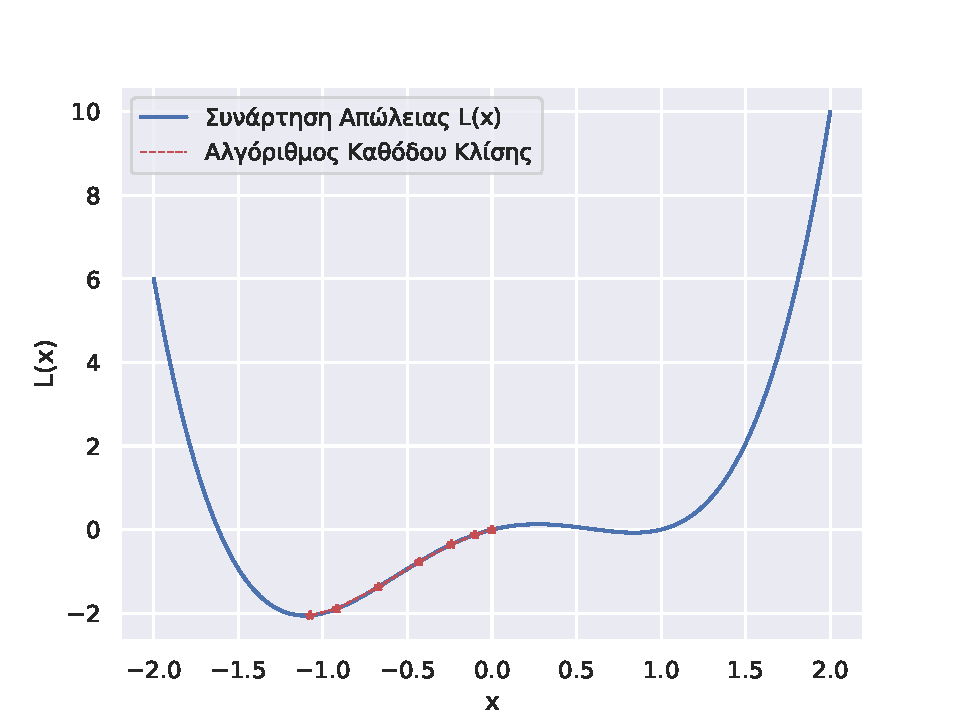
\includegraphics[width=0.7\textwidth]{images/chapter theoritical background/gd_init_at_plus0point1.pdf}
  \caption{Γραφική παράσταση στην οποία εφαρμόζεται ο αλγόριθμος καθόδου κλίσης σε μια μη κυρτή συνάρτηση με μια παράμετρο (την $x$). \todo[inline]{Να προσθέσω λινκ σε κώδικα.} Παράχθηκε τοπικά. }
  \label{fig:_gd01}
\end{figure}

Ο πιο δημοφιλής αλγόριθμος για αυτόν τον σκοπό είναι ο αλγόριθμος καθόδου κλίσης (\en{gradient descent}). Σύμφωνα με τον αλγόριθμο αυτό, πραγματοποιούνται επαναλαμβανόμενα βήματα \textquote{καθόδου} προς την κατεύθυνση με τη μεγαλύτερη κλίση. Διαισθητικά, φαίνεται λογικό σε κάθε βήμα να υπολογίζουμε σημειακά την κλίση της συνάρτησης που θέλουμε να ελαχιστοποιήσουμε και να κινούμαστε προς την κατεύθυνση με τη μικρότερη κλίση. Πιο συγκεκριμένα, πρώτα αρχικοποιούνται ανεξάρτητα όλες οι παράμετροι σε τυχαίες τιμές $\overline{W}_0$, $\overline{b}_0$ και έπειτα ξεκινά μια επαναληπτική διαδικασία όπου σε κάθε βήμα αυτής (έστω $i$):
\begin{enumerate}
  \item Υπολογίζονται οι μερικοί παράγωγοι (η κλήση) της συνάρτησης απώλειας ως προς όλες τις παραμέτρους σημειακά:
    \begin{equation}
      dw_i = \left.\frac{\partial \mathsf{L(\overline{W},\overline{b})}}{\partial w}\right\rvert_{(\overline{W},\overline{b})=(\overline{W}_{i-1},\overline{b}_i-1)}, \forall{w}
    \end{equation}
    και
    \begin{equation}
    db_i = \left.\frac{\partial \mathsf{L(\overline{W},\overline{b})}}{\partial b}\right\rvert_{(\overline{W},\overline{b})=(\overline{W}_{i-1},\overline{b}_i-1)}, \forall{b}
    \end{equation}
    Όπου $\mathsf{L(\overline{W},\overline{b})}$ η συνάρτηση απώλειας υπολογισμένη για ένα σύνολο δεδομένων $\boldsymbol{X}$ υπό τις παραμέτρους $\overline{W},\overline{b}$.
    Συνοπτικά, αν συγκεντρώσουμε όλες τις παραμέτρους $\overline{W}$ και $\overline{b}$ στο διάνυσμα στήλη $\overline{W_{all}}$ τότε γράφουμε:
    \begin{equation}
      {d \overline{W_{all}}}_i = \left.\nabla{\mathsf{L(\overline{W_{all}})}}\right\rvert_{\overline{W_{all}}=\overline{W_{all}}_{i-1}}
    \end{equation}
  \item Μετακινείται το σημείο στον χώρο παραμέτρων προς την κατεύθυνση της μεγαλύτερης κλίσης σύμφωνα με τον κανόνα ενημέρωσης (\en{update rule}) των παραμέτρων\footnote{Φανταστείτε τις παραγώγους ως \textquote{ευθύνες} της κάθε παραμέτρου για τις σωστές ή λάθος προβλέψεις. Όσο πιο μεγάλη η παράγωγος, τόσο πιο καθοριστικό ρόλο παίζει η μεταβλητή στη διαμόρφωση της τιμής της συνάρτησης απώλειας.}. Ο κανόνας είναι ο εξής:
  \begin{equation}
    w_i = w_{i-1} - \alpha \times dw_i, \forall{w} \end{equation}
    και
    \begin{equation} b_i = b_{i-1} - \alpha \times db_i, \forall{b}
    \end{equation}
    Όπου $\alpha$ ο ρυθμός μάθησης (\en{learning rate}): μια υπερπαράμετρος που καθορίζει το μέγεθος του βήματος κατά την ενημέρωση των παραμέτρων. Αντίστοιχα με πριν, συνοπτικά, έχουμε:
    \begin{equation}
      {\overline{W_{all}}}_i = {\overline{W_{all}}}_{i-1} - \alpha \times {d \overline{W_{all}}}_i
    \end{equation}
\end{enumerate} 
Ο αλγόριθμος τελειώνει είτε όταν οι ενημερώσεις είναι πλέον αμελητέες και η τιμή της συνάρτησης απώλειας δε μειώνεται άλλο από επανάληψη σε επανάληψη (ο αλγόριθμος έχει βρει ένα τοπικό ελάχιστο) είτε όταν ξεπεραστεί ο μέγιστος αριθμός επαναλήψεων.\par

\begin{figure}[h]
  \centering
  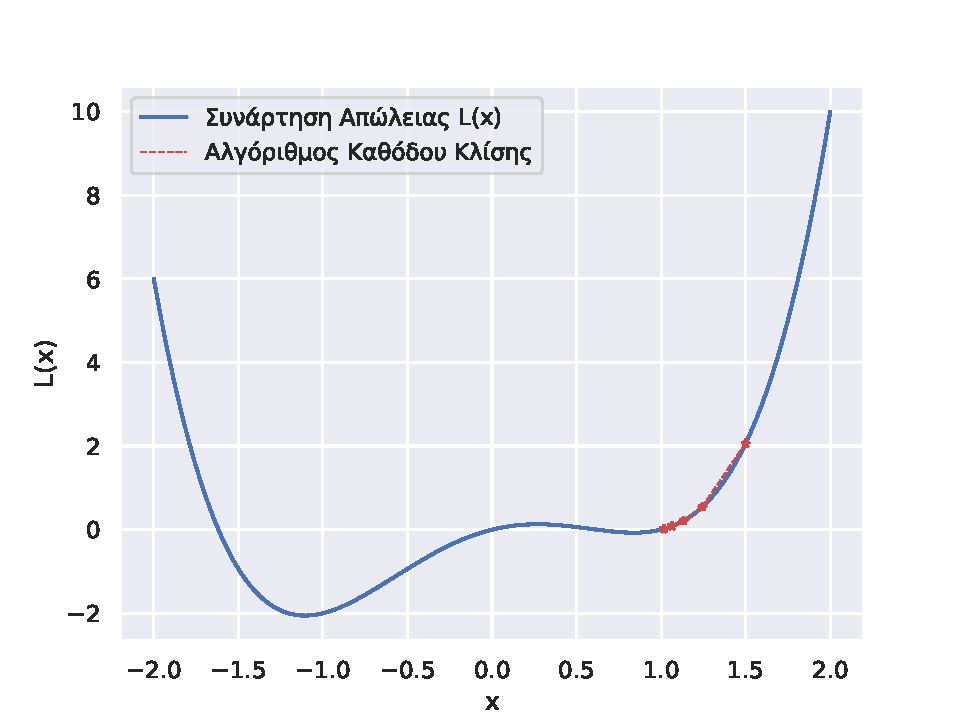
\includegraphics[width=0.7\textwidth]{images/chapter theoritical background/gd_init_at_plus1point5.pdf}
  \caption{Γραφική παράσταση στην οποία εφαρμόζεται ο αλγόριθμος καθόδου κλίσης σε μια μη κυρτή συνάρτηση με μια παράμετρο (την $x$) αρχικοποιημένη όμως στην τιμή 1.5 με αποτέλεσμα να βρίσκεται ένα τοπικό ελάχιστο.}
  \label{fig:_gd15}
\end{figure}

Να σημειώσουμε ότι ο αλγόριθμος καθόδου κλίσης δε βρίσκει πάντα το ολικό ελάχιστο της συνάρτησης. Ανάλογα με την αρχικοποίηση των παραμέτρων και τις τιμές των υπερπαραμέτρων (ρυθμός μάθησης, αριθμός επαναλήψεων) οδηγούμαστε κάθε φορά σε διαφορετικά αποτελέσματα. Για παράδειγμα, στο σχήμα \ref{fig:_gd15} αρχικοποιήσαμε την τιμή της παραμέτρου $x$ με την τιμή +1.5 με αποτέλεσμα ο αλγόριθμος να τερματίσει στο τοπικό ελάχιστο της συνάρτησης. Ανεξάρτητα από τον αριθμό επαναλήψεων, δε θα εντόπιζε ποτέ το ολικό ελάχιστο υπό αυτήν την αρχικοποίηση. Η αδυναμία εγγύησης για την εύρεση του ολικού ελαχίστου αποτελεί τον λόγο για τον οποίο σε αρκετά προβλήματα μηχανικής μάθησης οι αλγόριθμοι εκπαιδεύονται πολλές φορές με διαφορετική όμως αρχικοποίηση των παραμέτρων τους. Ευτυχώς, στα πολυεπίπεδα νευρωνικά δίκτυα δεν ενδιαφέρει η εύρεση του ολικού ελαχίστου\footnote{Καθώς οδηγεί σε \en{overfitting}.} αλλά ενός τοπικού ελαχίστου \cite{choromanska2015loss}.\par

Ο αλγόριθμος της καθόδου κλίσης δε θα χρησίμευε στην εκπαίδευση των νευρωνικών δικτύων αν δεν υπήρχε η δυνατότητα αποδοτικού υπολογισμού των μερικών παραγώγων. Ευτυχώς, τη λειτουργία αυτή την επιτελεί η μέθοδος οπισθοδιάδοσης σφάλματος (\en{back propagation}). Με λίγα λόγια, πρόκειται για μια μέθοδο η οποία χρησιμοποιώντας τον κανόνα της αλυσίδας υπολογίζει την παράγωγο της συνάρτησης απώλειας ως προς όλες τις παραμέτρους του δικτύου (σημειακά), ξεκινώντας από αυτές του τελευταίου επιπέδου και τερματίζοντας σε αυτές του πρώτου.\par

Παρακάτω παρατίθενται οι υπολογισμοί που λαμβάνουν χώρα κατά τη διάρκεια εύρεσης των μερικών παραγώγων ως προς τις παραμέτρους ενός επιπέδου $L-1$ μέσω της οπισθοδιάδοσης σφάλματος για την $i$\textendash οστή επανάληψη του αλγορίθμου καθόδου κλίσης. Αν και οι παράγωγοι υπολογίζονται σημειακά για τις τιμές των παραμέτρων $\overline{W}_i$ και $\overline{b}_i$, για λόγους ευκολότερης ανάγνωσης αυτό δε θα απεικονίζεται κατά τη διατύπωση των παρακάτω μερικών παραγώγων. Ξεκινώντας από το επίπεδο $L$ έχουμε:
\begin{itemize}
  \item Η παράγωγος της συνάρτησης απώλειας ως προς τα βάρη από τον κόμβο $k$ του επιπέδου $L-1$ ston κόμβο $j$ του επιπέδου $L$ είναι:
  \begin{equation}\label{eq:dw}
    \frac{\partial \mathsf{L(\overline{W},\overline{b})}}{{\partial w^{[L]}_{jk}}} = 
    \frac{\partial \mathsf{z_j^{[L]}}}{{\partial w^{[L]}_{jk}}} \times
    \frac{\partial \mathsf{a_j^{[L]}}}{{\partial z_j^{[L]}}} \times
    \frac{\partial \mathsf{L(\overline{W},\overline{b})}}{{\partial a^{[L]}_{j}}}
  \end{equation}
  Όπου ο όρος $\frac{\partial \mathsf{L(\overline{W},\overline{b})}}{{\partial a^{[L]}_{j}}}$ υπολογίζεται άμεσα από την επιλεγμένη συνάρτηση απώλειας.\\ 
  Ο όρος $\frac{\partial \mathsf{a_j^{[L]}}}{{\partial z_j^{[L]}}}$ υπολογίζεται άμεσα από την επιλεγμένη συνάρτηση ενεργοποίησης.\\
  Τέλος, η μερική παράγωγος $\frac{\partial \mathsf{z_j^{[L]}}}{{\partial w^{[L]}_{jk}}}$ υπολογίζεται λαμβάνοντας την παράγωγο του γραμμικού συνδυασμού 
  \item Η παράγωγος της συνάρτησης απώλειας ως προς τα δυναμικά πόλωσης είναι:
  \begin{equation}\label{eq:db}
    \frac{\partial \mathsf{L(\overline{W},\overline{b})}}{{\partial b^{[L]}_{j}}} = 
    \frac{\partial \mathsf{z_j^{[L]}}}{{\partial b^{[L]}_{j}}} \times
    \frac{\partial \mathsf{a_j^{[L]}}}{{\partial z_j^{[L]}}} \times
    \frac{\partial \mathsf{L(\overline{W},\overline{b})}}{{\partial a^{[L]}_{j}}}
  \end{equation}
  Στην περίπτωση αυτή, η μερική παράγωγος $\frac{\partial \mathsf{z_j^{[L]}}}{{\partial b^{[L]}_{j}}} = 1$.
  \item Τέλος, η παράγωγος της συνάρτησης απώλειας ως προς τις τιμές ενεργοποίησης του προηγούμενου επιπέδου $a^{[L-1]}_{k}$ είναι:
  \begin{equation}\label{eq:da L-1}
    \frac{\partial \mathsf{L(\overline{W},\overline{b})}}{{\partial a^{[L-1]}_{k}}} = 
\sum_{j = 1}^{n^{[L]}}     \frac{\partial \mathsf{z_j^{[L]}}}{{\partial a^{[L-1]}_{k}}} \times
    \frac{\partial \mathsf{a_j^{[L]}}}{{\partial z_j^{[L]}}} \times
    \frac{\partial \mathsf{L(\overline{W},\overline{b})}}{{\partial a^{[L]}_{j}}} 
  \end{equation}

\end{itemize}
Παρατηρούμε ότι οι μερικοί παράγωγοι των μεταβλητών ενός επιπέδου $l-1$ εξαρτώνται από το επίπεδο $l$. Για αυτό και όπως προαναφέραμε, οι υπολογισμοί ξεκινούν από το τελευταίο επίπεδο. Επαγωγικά, με τη χρήση της \ref{eq:da L-1} στις \ref{eq:dw} και \ref{eq:db} μπορούμε να βρούμε τις μερικές παραγώγους ως προς τις παραμέτρους όλων των επιπέδων.\par

Συγκεντρωτικά, χρησιμοποιώντας την αναπαράσταση με χρήση πίνακα που παρουσιάσαμε στην προηγούμενη παράγραφο, οι σχέσεις \ref{eq:dw}, \ref{eq:db} και \ref{eq:da L-1} γράφονται αντίστοιχα:
\begin{equation}\label{eq:_bw}
  \frac{\partial \mathsf{L(\overline{W},\overline{b})}}{{\partial \boldsymbol{W}^{[l]}}} = \frac{1}{M} \times \big(\frac{\partial \mathsf{L(\overline{W},\overline{b})}}{\partial \boldsymbol{A}^{[l]}} \odot \frac{\partial \mathsf{{\boldsymbol{A}^{[l]}}}}{\partial \boldsymbol{Z}^{[l]}} \big) \times {\boldsymbol{A}^{[l-1]}}^T
\end{equation}
\begin{equation}\label{eq:_bb}
  \frac{\partial \mathsf{L(\overline{W},\overline{b})}}{\partial \boldsymbol{b}^{[l]}} = \frac{1}{M} \times \big(\frac{\partial \mathsf{L(\overline{W},\overline{b})}}{\partial \boldsymbol{A}^{[l]}} \odot \frac{\partial \mathsf{{\boldsymbol{A}^{[l]}}}}{\partial \boldsymbol{Z}^{[l]}} \big) \times \boldsymbol{1}_M^T
\end{equation}
\begin{equation}\label{eq:_ba}
  \frac{\partial \mathsf{L(\overline{W},\overline{b})}}{{\partial \boldsymbol{A}^{[l-1]}}} =  {\boldsymbol{W}^{[l]}}^T\times \big(\frac{\partial \mathsf{L(\overline{W},\overline{b})}}{\partial \boldsymbol{A}^{[l]}} \odot \frac{\partial \mathsf{{\boldsymbol{A}^{[l]}}}}{\partial \boldsymbol{Z}^{[l]}} \big) 
\end{equation}

Όπου ο τελεστής $\odot$ συμβολίζει το γινόμενο στοιχείο προς στοιχείο (\en{elementwise product}) ενώ το $\boldsymbol{1}_n = \big[1, 1, 1, \dots, 1\big] \in \Re^n$. Για τον όρο στην παρένθεση που συναντάται συχνά στους ανωτέρω τύπους ισχύει $\big(\frac{\partial \mathsf{L(\overline{W},\overline{b})}}{\partial \boldsymbol{A}^{[l]}} \odot \frac{\partial \mathsf{{\boldsymbol{A}^{[l]}}}}{\partial \boldsymbol{Z}^{[l]}} \big) = \frac{\partial \mathsf{L(\overline{W},\overline{b})}}{{\partial \boldsymbol{Z}^{[l]}}}$. \par

Σαν τελικά σχόλια σχετικά με την εκπαίδευση των νευρωνικών δικτύων είναι ωφέλιμο να κάνουμε δύο παρατηρήσεις:
\begin{itemize}
  \item Κατά την εφαρμογή του αλγορίθμου καθόδου κλίσης σε ένα νευρωνικό δίκτυο, σε κάθε βήμα αυτού γίνονται δύο περάσματα: μια πρόσθια διάδοση που περιγράφεται από τις εξισώσεις \ref{eq:_fw_z} και \ref{eq:fw_a} για τον υπολογισμό της συνάρτησης απώλειας και μια οπισθοδιάδοση που περιγράφεται από τις εξισώσεις \ref{eq:_bw}, \ref{eq:_bb} και \ref{eq:_ba} για τον υπολογισμό των παραγώγων που χρησιμοποιούνται στον κανόνα ενημέρωσης.
  \item Επειδή το σύνολο δεδομένων εισόδου μπορεί να είναι πολύ μεγάλο, αντί να λαμβάνονται όλα τα παραδείγματα Μ για τον υπολογισμό του $d\overline{W_{all}}$ με βάση τη συνάρτησης απώλειας, συνηθίζεται να χωρίζεται σε μικρά πακέτα (\en{mini batches}) από $m$ παραδείγματα το καθένα. Έτσι, πραγματοποιείται ένα βήμα ενημέρωσης για κάθε μικρό πακέτο δεδομένων. Όταν εφαρμόζεται αυτή η τακτική, σιωπηρά γίνεται η υπόθεση ότι το κάθε δείγμα των $m$ παραδειγμάτων είναι επαρκώς αντιπροσωπευτικό ώστε η συνάρτηση απώλειας υπολογισμένη στα $m$ παραδείγματα να είναι καλή προσέγγιση της συνάρτησης υπολογισμένης στα $M$ παραδείγματα. Ακραία μορφή αυτού είναι ο στοχαστικός αλγόριθμος καθόδου κλίσης (\en{stochastic gradient descent}) στον οποίο $m=1$. Οι μαθηματικοί τύποι που παραθέσαμε σε αυτό το κεφάλαιο ισχύουν σε κάθε περίπτωση μετά την κατάλληλη ανάθεση της υπερπαραμέτρου $M$.
\end{itemize}

\subsubsection{Συνελικτικά Νευρωνικά Δίκτυα}

Έχοντας περιγράψει τη δομή και την εκπαίδευση των απλών νευρωνικών δικτύων πρόσθιας διάδοσης, εύκολα μπορούμε να κατανοήσουμε μερικές από τις παραλλαγές του. Μια από τις σημαντικότερες παραλλαγές είναι αυτή των Συνελικτικών Νευρωνικών Δικτύων (\en{Convolutional Neural Networks}) που χρησιμοποιείται συστηματικά στον χώρο της όρασης υπολογιστών. Πρόκειται για την υποκατηγορία των νευρωνικών δικτύων πρόσθιας διάδοσης στην οποία οδηγήθηκε η επιστημονική κοινότητα αφενός επιδιώκοντας να λύσει ορισμένα από τα πρακτικά προβλήματα της εφαρμογής νευρωνικών δικτύων στον χώρο της όρασης υπολογιστών και αφετέρου μελετώντας τη νεύρο\textendash φυσιολογία του οπτικού φλοιού (\en{visual cortex}).\par

Από τη σκοπιά της νευροεπιστήμης, οι \en{David H. Hubel} και \en{Torsten Wiesel} μετά από μια σειρά πειραμάτων σε γάτες \cite{hubel1959single, hubel1959receptive} γύρω στο 1960 και αργότερα, σε πιθήκους \cite{hubel1968receptive} έριξαν φως στη δομή του οπτικού φλοιού, εμπνέοντας έτσι το κίνημα του διασυνδετισμού (\en{connectionism}). Σύμφωνα με το έργο τους (για το οποίο τιμήθηκαν με το βραβείο \en{nobel} το 1981) πολλοί νευρώνες του οπτικού φλοιού έχουν μικρά, τοπικά πεδία υποδοχής (\en{receptive fields}) που μπορεί να επικαλύπτονται μεταξύ τους. Με άλλα λόγια, ο κάθε νευρώνας αφορά ένα περιορισμένο τμήμα του οπτικού πεδίου αλλά όλοι μαζί, καλύπτουν το σύνολό του. Επιπλέον, μετά από πειράματα οπτικής αναγνώρισης σχημάτων (οριζόντιο παραλληλόγραμμο σε μορφή μπάρας) σε διάφορες γεωμετρίες παρατηρήθηκε ότι διαφορετικοί νευρώνες με το ίδιο πεδίο υποδοχής ενεργοποιούνται ανάλογα με τη γεωμετρία του σχήματος (κάποιοι νευρώνες ενεργοποιούνται κατά τον κάθετο προσανατολισμό της μπάρας ενώ άλλοι με τον οριζόντιο προσανατολισμό της). Τέλος, επισήμαναν ότι ορισμένοι νευρώνες ενεργοποιούνται με την αναγνώριση πιο περίπλοκων μοτίβων όπως προκύπτουν από τη σύνθεση απλών γεωμετριών χαμηλότερου επιπέδου \cite{geron2019hands}. \par
 
Από πρακτικής σκοπιάς, η τροφοδότηση ενός . Για παράδειγμα έστω εικόνα .... Έπρεπε να βρεθεί πιο αποδοτικός τρόπος.

Από τις παραπάνω απαιτήσεις, εμπνεόμενες από το ... γέννησαν τα συνελικτικά νευρωνικά δίκτυα...  weight sharing... βλ σχήμα... μέγιστη συνάθριση ... συνελικτικό επίπεδο\dots ... feature extraction...

Συνελικτικό επίπεδο

Υποδειγματοληψία...
Συνολικά παράμετροι\dots

\begin{figure}[h]
  \centering
  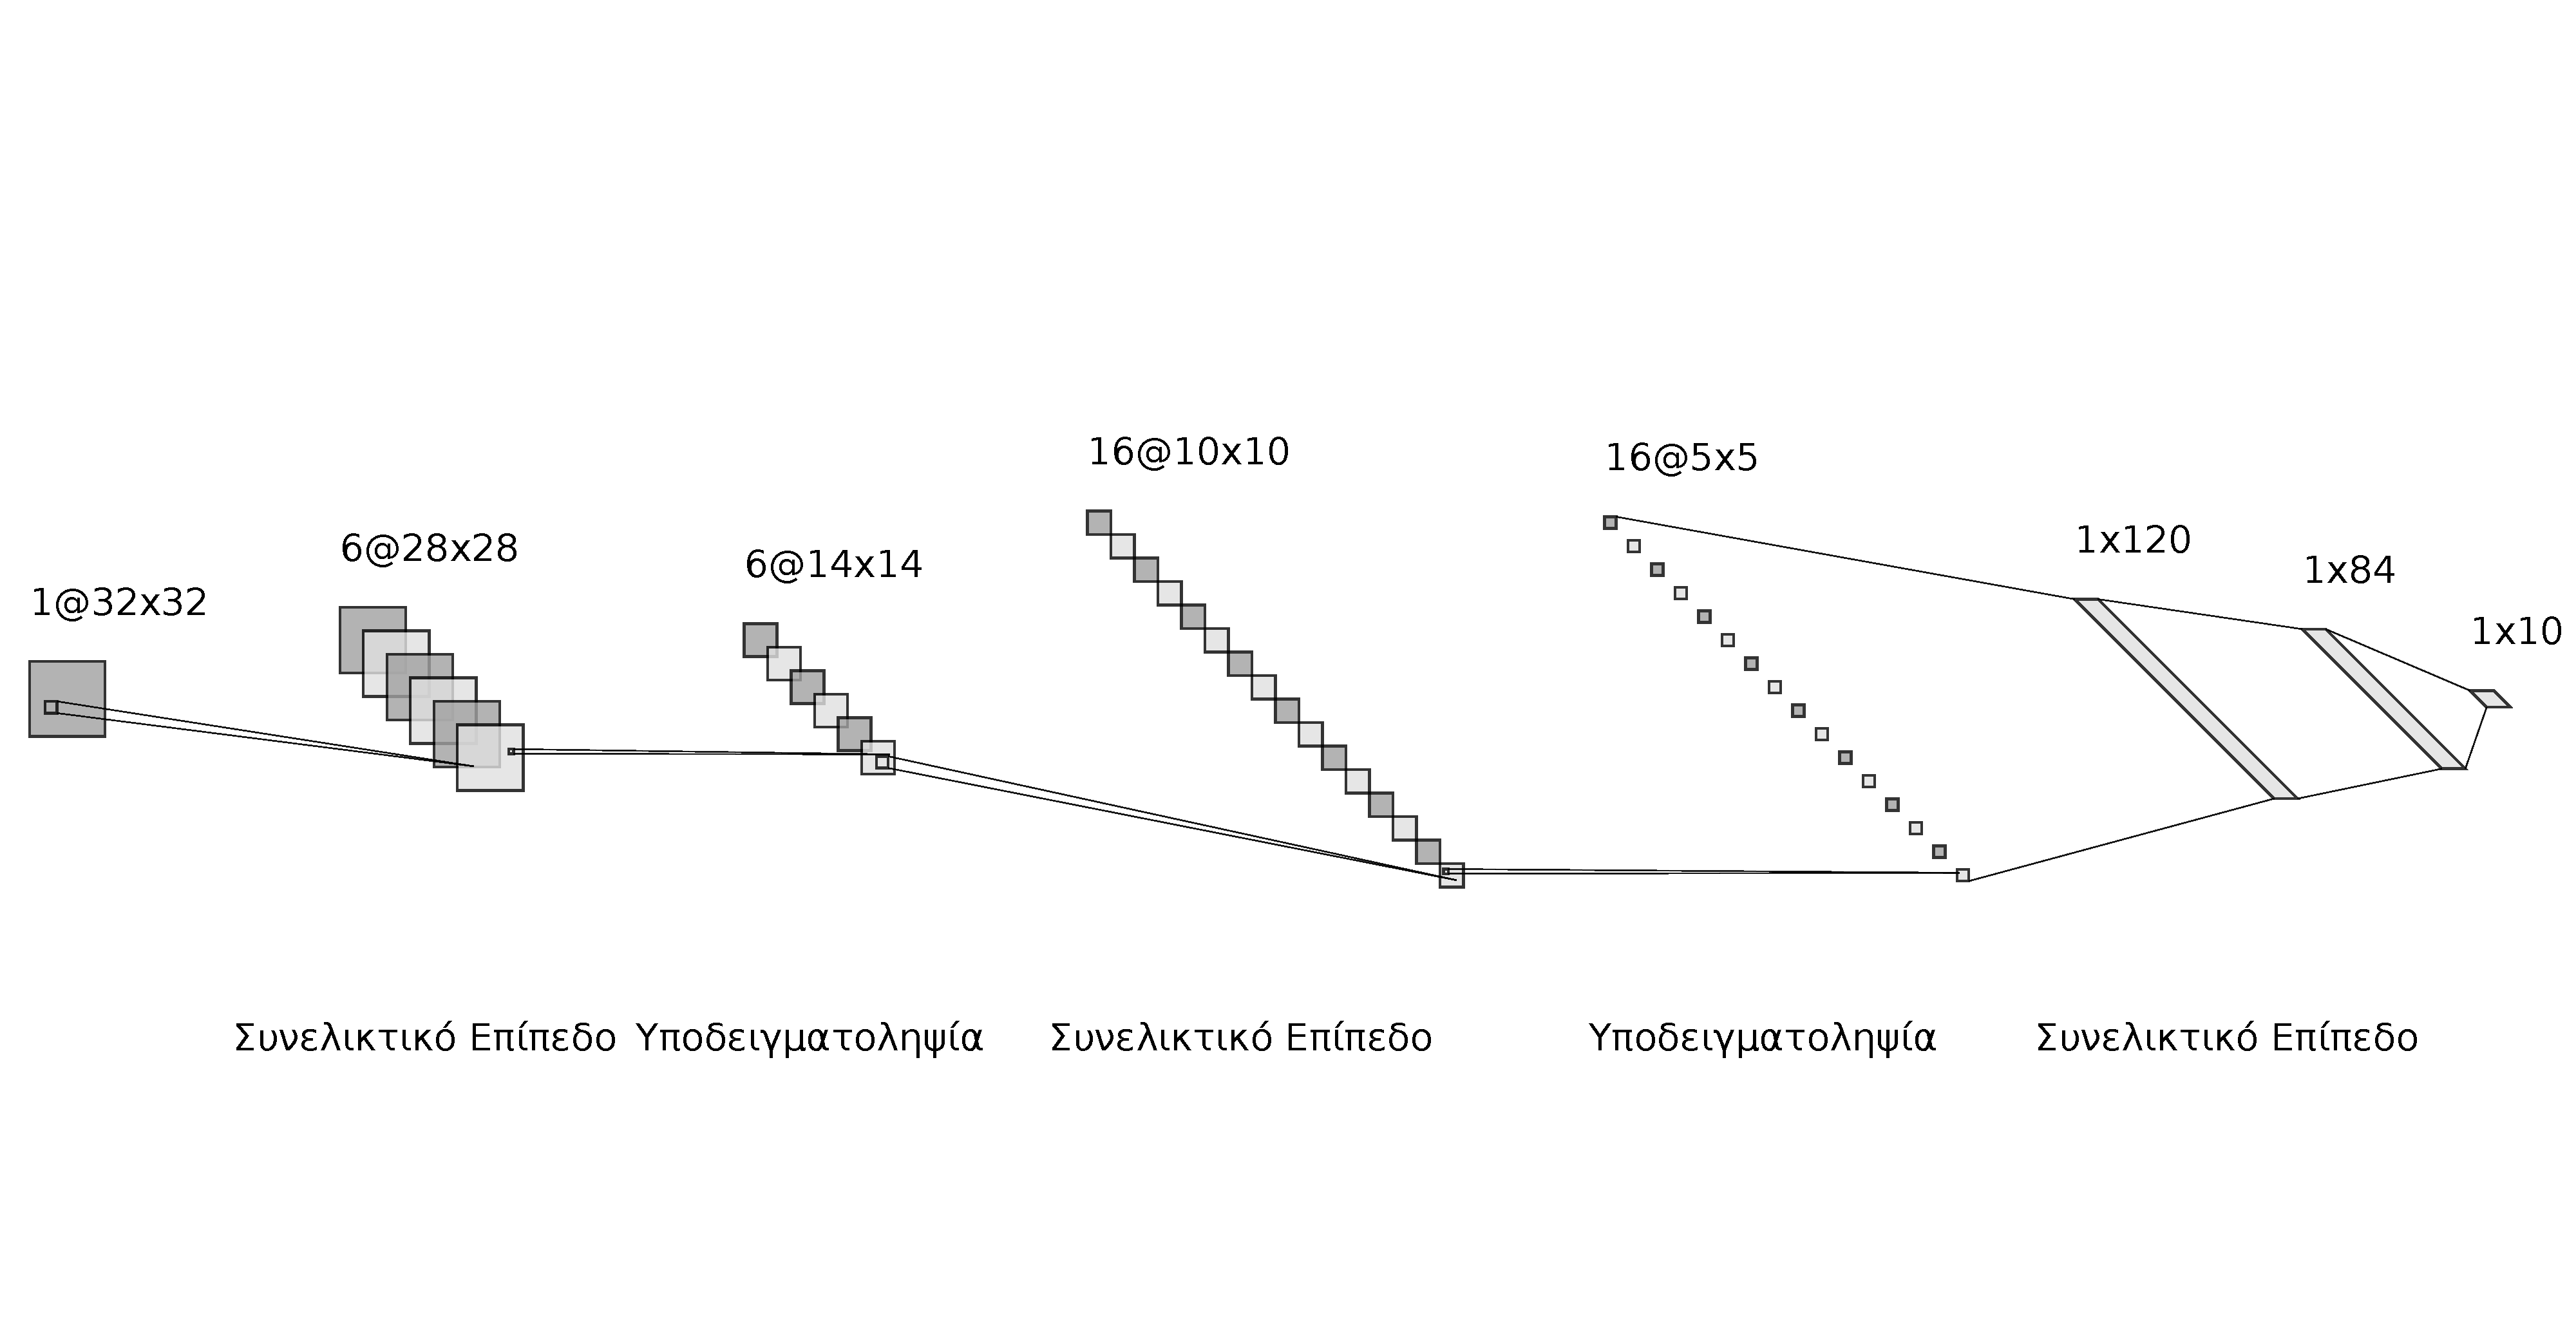
\includegraphics[width=0.9\textwidth]{images/chapter theoritical background/lenet-greek-new.pdf}
  \caption{Αρχιτεκτονική Συνελικτικού Νευρωνικού Δικτύου \cite{lenet}. \textit{Παράχθηκε από το \href{http://alexlenail.me/NN-SVG/LeNet.html}{\en{NN-SVG}}.}}
  \label{fig:_nn_lenet}
\end{figure}
\subsubsection{Στρατηγικές Βελτίωσης Απόδοσης Νευρωνικών Δικτύων}
\section{Νευρωνικά Δίκτυα με Κάψουλες}
\section{Μηχανισμός Προσοχής}
\section{Μετασχηματιστές}
\section{Χάρτες Αυτο-οργάνωσης}
\label{sec:_SOM}
\section{Αλγόριθμος \en{EM}}
\label{sec:_EM}
\section{Συμπερασματολογία μέσω Διακύμανσης}
% autoencoders